\chapter{Optimisation de la parallélisation}
\par
Malheureusement, nous n'avons pas implémenté les cellules fantômes, mais pour l'optimisation parallèle, nous avons changé le mode d'utilisation de MPI\_Send et MPI\_Recv (envoi et réception) dans la deuxième question en utilisant MPI\_Bcast (mode de diffusion) et avons obtenu une amélioration des performances.\begin{figure}[h]
    \centering
    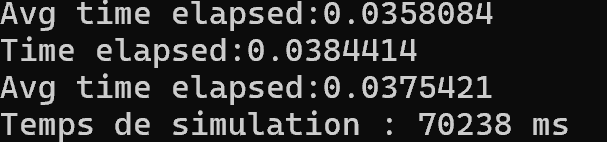
\includegraphics[width=0.9\linewidth]{mpi_broadcast.png}
    \caption{MPI boardcast}
    \label{fig:enter-label}
\end{figure}
\par C'est parce que le mode de diffusion garantit que tous les processus peuvent continuer à exécuter l'étape suivante après avoir reçu les données de diffusion. Tous les processus seront traités de manière synchrone une fois la diffusion des données terminée, évitant ainsi les situations asynchrones. 
Mais dans les modes MPI\_Send et MPI\_Recv, la gestion de la synchronisation entre les processus nécessite du code supplémentaire pour garantir que chaque processus reçoit les données à temps, ce qui peut entraîner des problèmes de synchronisation plus complexes, en particulier lorsque le nombre de processus est important.